\documentclass[border=2pt]{standalone}
\usepackage{tikz}
\usetikzlibrary{fadings}

\begin{document}
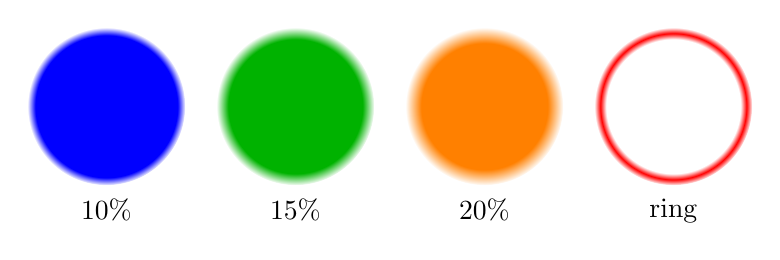
\begin{tikzpicture}
  \fill[blue,path fading=circle with fuzzy edge 10 percent] (0,0) circle (1cm);
  \fill[green!70!black,path fading=circle with fuzzy edge 15 percent] (2.4,0) circle (1cm);
  \fill[orange,path fading=circle with fuzzy edge 20 percent] (4.8,0) circle (1cm);
  \fill[red,path fading=fuzzy ring 15 percent] (7.2,0) circle (1cm);
  \node[below] at (0,-1.05) {10\%};
  \node[below] at (2.4,-1.05) {15\%};
  \node[below] at (4.8,-1.05) {20\%};
  \node[below] at (7.2,-1.05) {ring};
\end{tikzpicture}
\end{document}
